%%
%% This is file `tikzposter-template.tex',
%% generated with the docstrip utility.
%%
%% The original source files were:
%%
%% tikzposter.dtx  (with options: `tikzposter-template.tex')
%%
%% This is a generated file.
%%
%% Copyright (C) 2014 by Pascal Richter, Elena Botoeva, Richard Barnard, and Dirk Surmann
%%
%% This file may be distributed and/or modified under the
%% conditions of the LaTeX Project Public License, either
%% version 2.0 of this license or (at your option) any later
%% version. The latest version of this license is in:
%%
%% http://www.latex-project.org/lppl.txt
%%
%% and version 2.0 or later is part of all distributions of
%% LaTeX version 2013/12/01 or later.
%%


\documentclass{tikzposter} %Options for format can be included here

\usepackage{todonotes}

\usepackage[tikz]{bclogo}
\usepackage{lipsum}
\usepackage{amsmath}

\usepackage{booktabs}
\usepackage{longtable}
\usepackage[absolute]{textpos}
\usepackage[it]{subfigure}
\usepackage{graphicx}
\usepackage{cmbright}
%\usepackage[default]{cantarell}
%\usepackage{avant}
%\usepackage[math]{iwona}
\usepackage[math]{kurier}
\usepackage[T1]{fontenc}


%% add your packages here
\usepackage{hyperref}
% for random text
\usepackage{lipsum}
\usepackage[english]{babel}
\usepackage[pangram]{blindtext}

\colorlet{backgroundcolor}{blue!10}

 % Title, Author, Institute
\title{What's Cooking?}
\author{Jincai Ma}
\institute{ Xi'an Shiyou University, China \\
}
%\titlegraphic{logos/tulip-logo.eps}

%Choose Layout
\usetheme{Wave}

%\definebackgroundstyle{samplebackgroundstyle}{
%\draw[inner sep=0pt, line width=0pt, color=red, fill=backgroundcolor!30!black]
%(bottomleft) rectangle (topright);
%}
%
%\colorlet{backgroundcolor}{blue!10}

\begin{document}


\colorlet{blocktitlebgcolor}{blue!23}

 % Title block with title, author, logo, etc.
\maketitle

\begin{columns}
 % FIRST column
\column{0.5}% Width set relative to text width

%%%%%%%%%% -------------------------------------------------------------------- %%%%%%%%%%
 %\block{Main Objectives}{
%  	      	\begin{enumerate}
%  	      	\item Formalise research problem by extending \emph{outlying aspects mining}
%  	      	\item Proposed \emph{GOAM} algorithm is to solve research problem
%  	      	\item Utilise pruning strategies to reduce time complexity
%  	      	\end{enumerate}
%%  	      \end{minipage}
%}
%%%%%%%%%% -------------------------------------------------------------------- %%%%%%%%%%


%%%%%%%%%% -------------------------------------------------------------------- %%%%%%%%%%
\block{Introduction}{
  
  	
    \begin{description}
      
  	\item[The Data Source] The data comes from Kaggle https://www.kaggle.com/c/whats-cooking.
  	
  	\item[Project Purpose] Use recipe ingredients to categorize the cuisine.\\
      Given the name of the condiment, predict the cuisine to which the dish belongs.
    \item[Related Field Name Interpretation] In the dataset,  including the recipe ID, the dish, and the list of ingredients for each recipe (variable length).The data is stored in JSON format. \\
    1.train.json- A training set that contains the recipe ID, dish type, and ingredient list\\
    2.test.json- A test set containing a recipe ID and a list of ingredients\\
    3.sample\_submission.csv- Properly formatted sample submission document
  	\end{description}

  	
}
%%%%%%%%%% -------------------------------------------------------------------- %%%%%%%%%%


%%%%%%%%%% -------------------------------------------------------------------- %%%%%%%%%%

%%%%%%%%%% -------------------------------------------------------------------- %%%%%%%%%%

%%%%%%%%%% -------------------------------------------------------------------- %%%%%%%%%%
\block{ Data Import And Introduction}{
                                       
    \begin{itemize}
        \item
        Import the JSON file with Pandas:
        We can get the data set of dish names, including 39774 training data and 9944 test samples.
        \item To see the distribution of our data set and the total variety of dishes, we printed out some of the data samples.
    \end{itemize}
    \begin{minipage}{1\linewidth}
        \centering
        \includegraphics[width=1\textwidth]{pic1/1.png} 
    \end{minipage}

    \begin{itemize}
        \item
        Total dish classification\\
        There are 20 dishes in total, which are:
        ['brazilian' 'british' 'cajun\_creole' 'chinese' 'filipino' 'french'
         'greek' 'indian' 'irish' 'italian' 'jamaican' 'japanese' 'korean'
         'mexican' 'moroccan' 'russian' 'southern\_us' 'spanish' 'thai'
         'vietnamese']
        
    \end{itemize}
    
}
%%%%%%%%%% -------------------------------------------------------------------- %%%%%%%%%%
\block{Data Analysis}{
    
    \begin{itemize}                            
        \item The data set is divided into Features and Target Variables.
        \item Features:'ingredients', we were given the names of the ingredients contained in each dish.
        Target variable:'cuisine', is the classification of cuisines that we want to predict.
        
    \end{itemize}
    
    \begin{itemize}                            
        \item
        What are the top 10 most frequently used ingredients?
        \item What are the 10 most common ingredients in filipino,greek and Italian cuisine?
    \end{itemize}
    \begin{minipage}{0.5\linewidth}
        \centering
        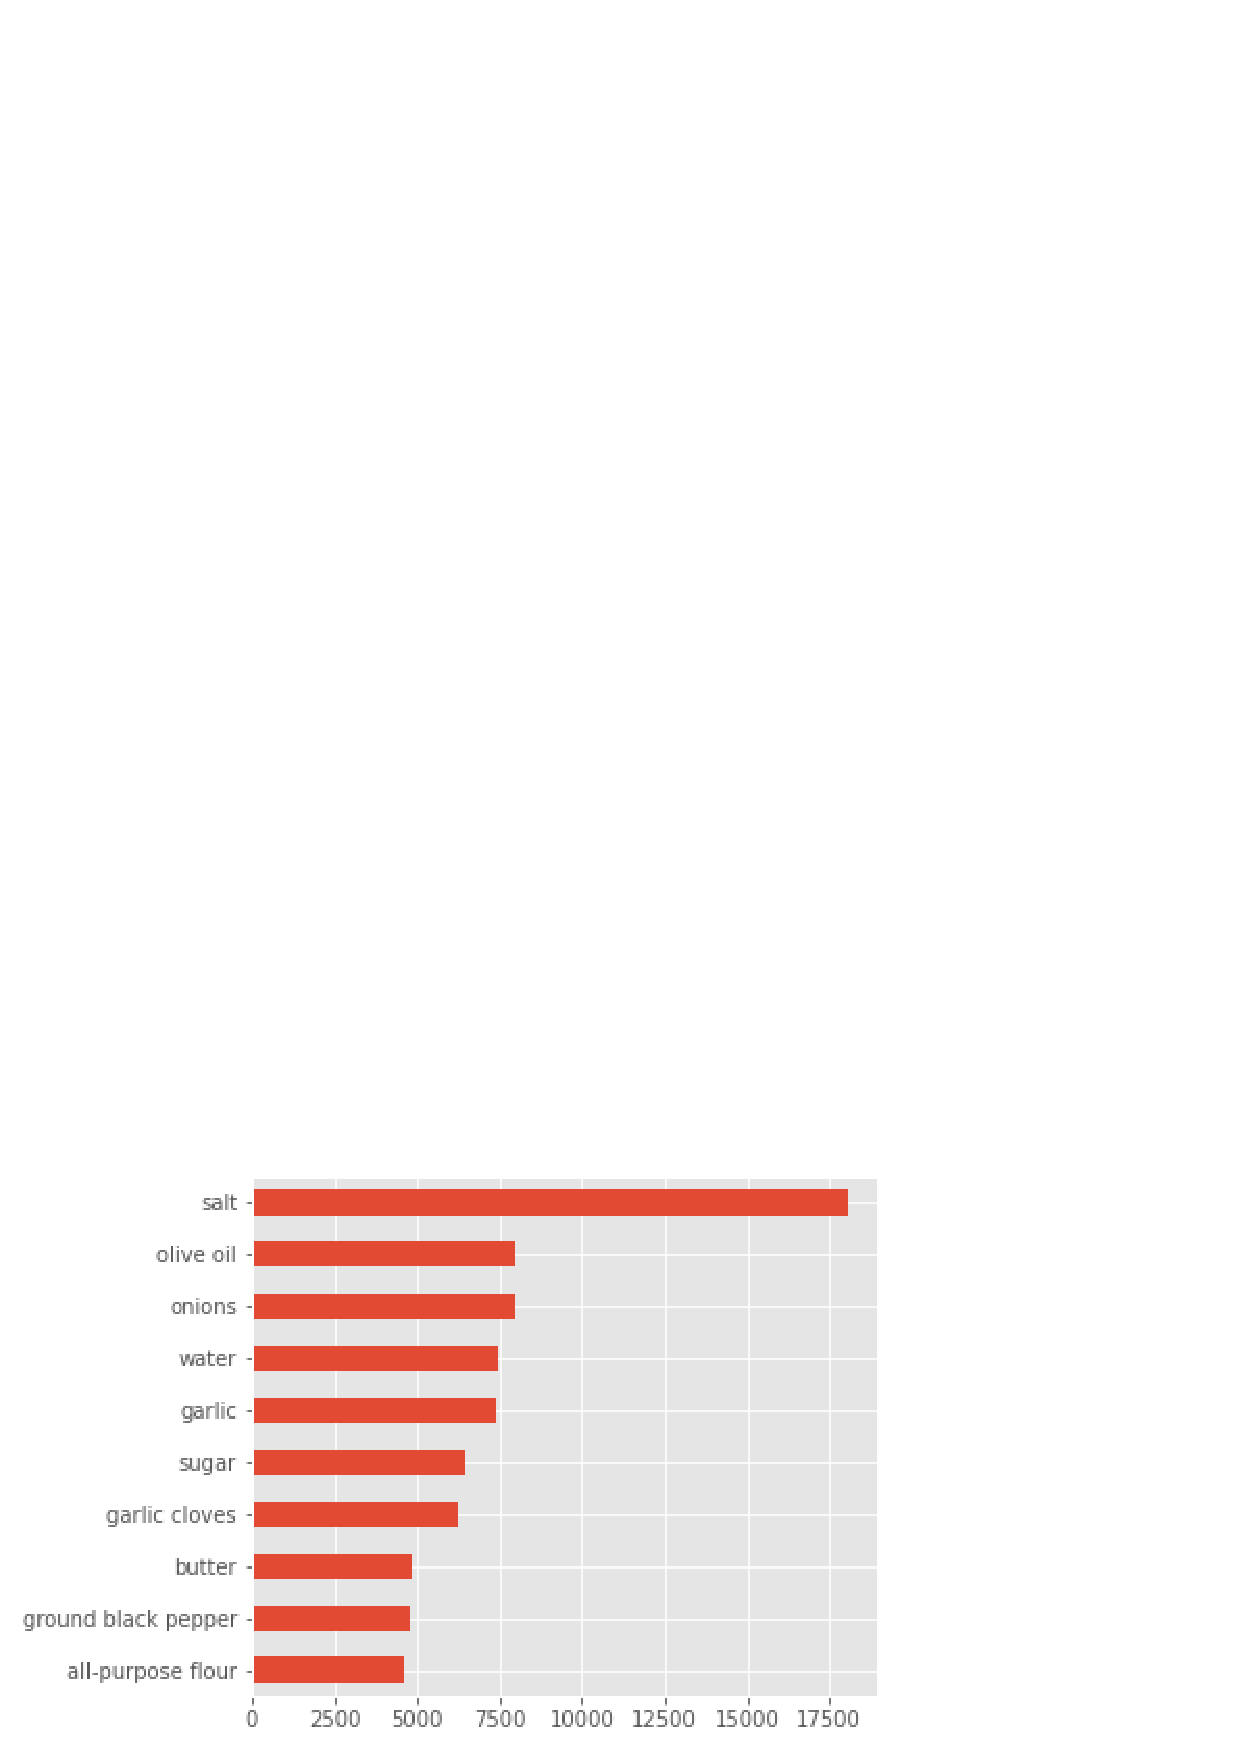
\includegraphics[width=0.5\textwidth]{pic1/cooking.png} 
    \end{minipage}
    \begin{minipage}{0.5\linewidth}
        \centering
        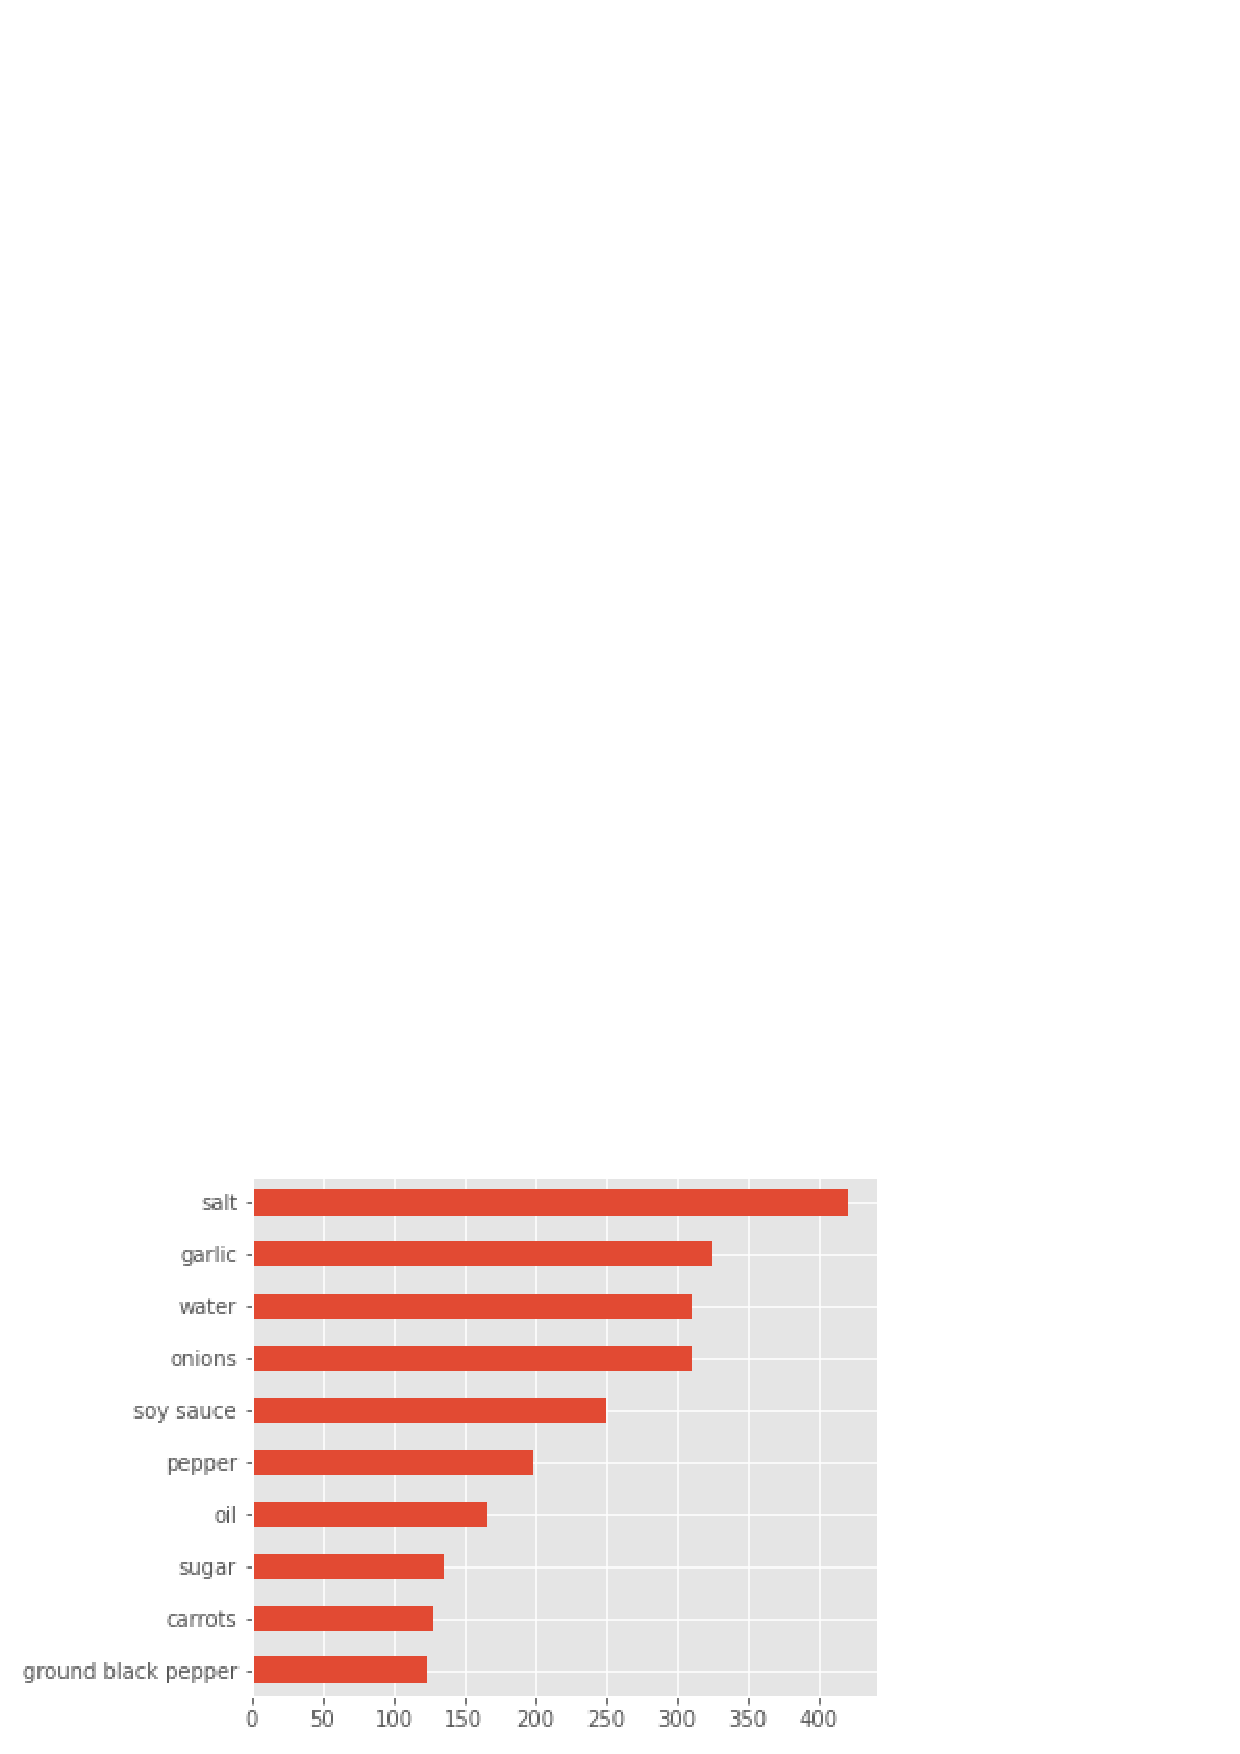
\includegraphics[width=0.5\textwidth]{pic1/filipino.png} 
    \end{minipage}
    \begin{minipage}{0.5\linewidth}
        \centering
        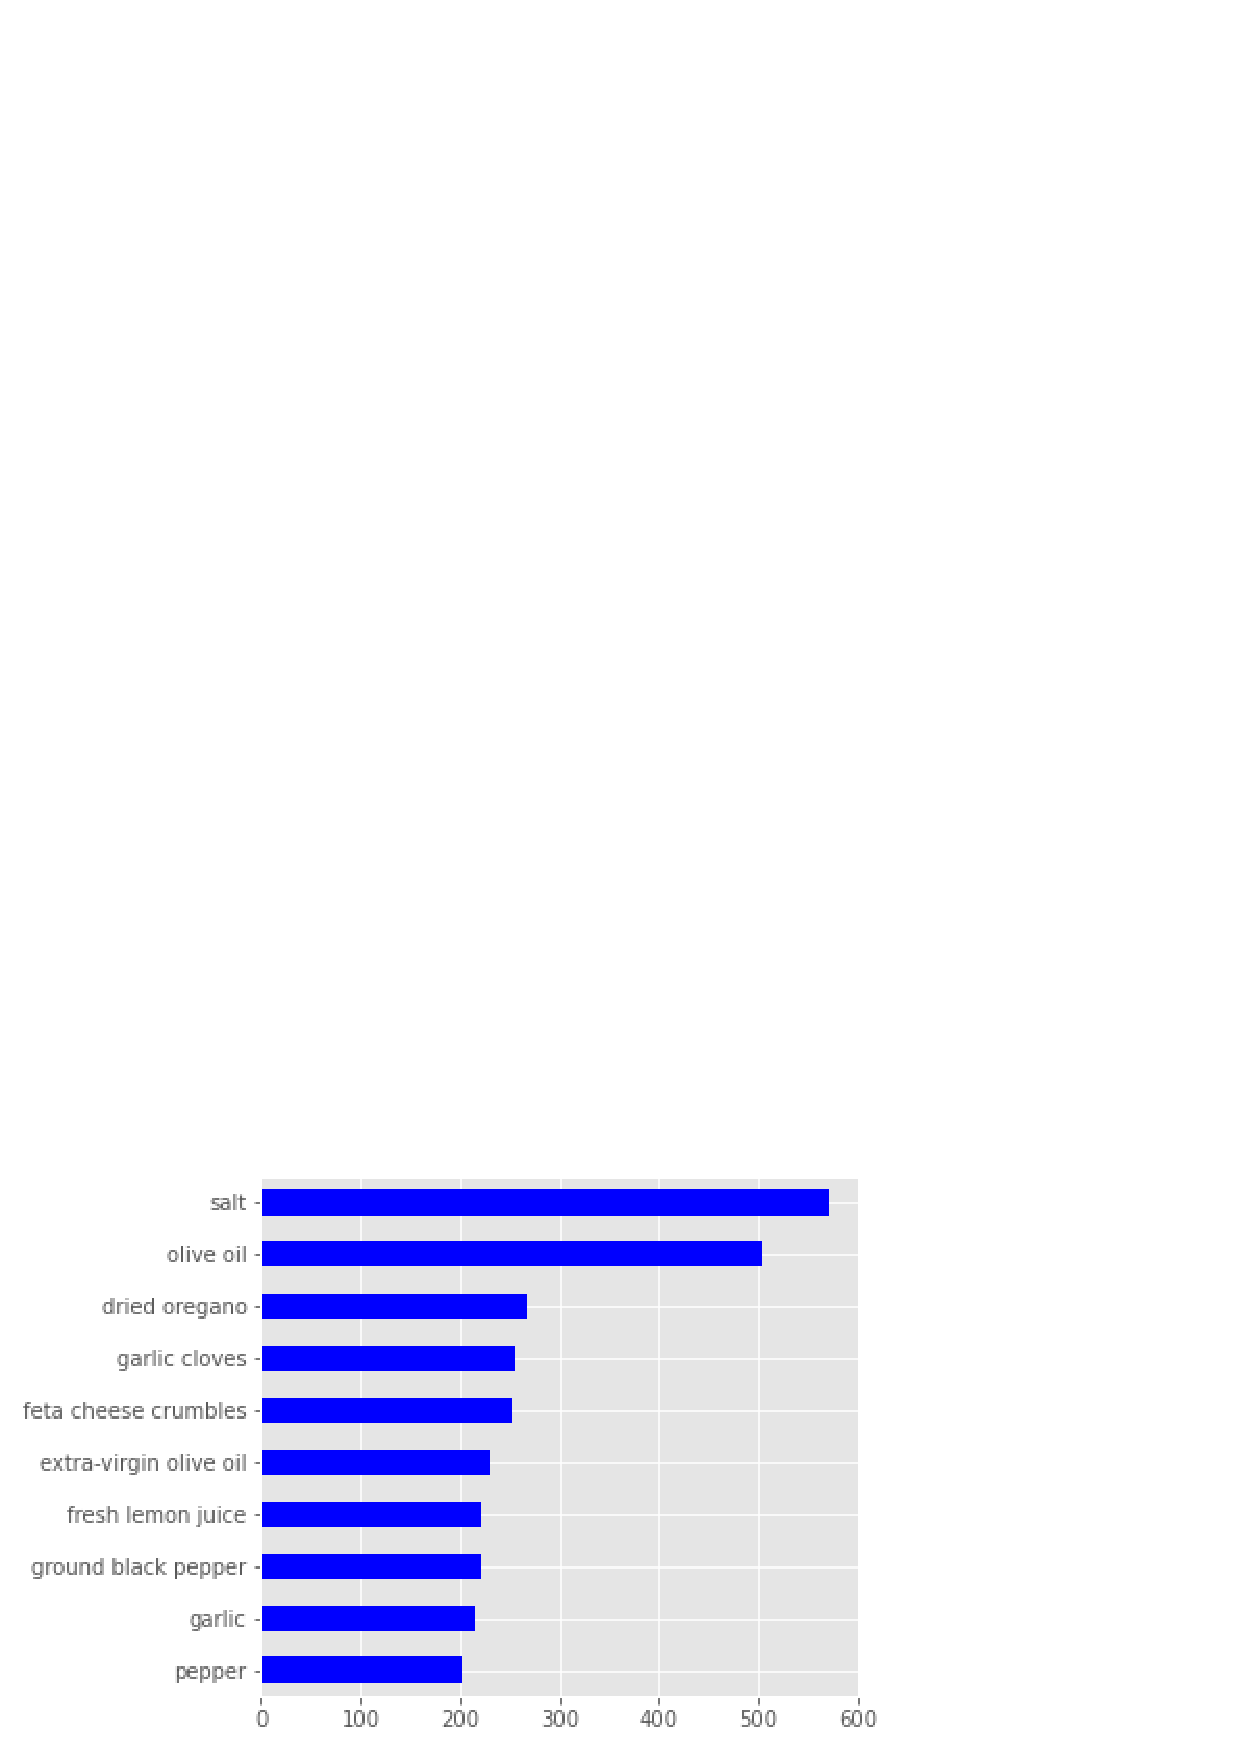
\includegraphics[width=0.5\textwidth]{pic1/greek.png} 
    \end{minipage}
    \begin{minipage}{0.5\linewidth}
        \centering
        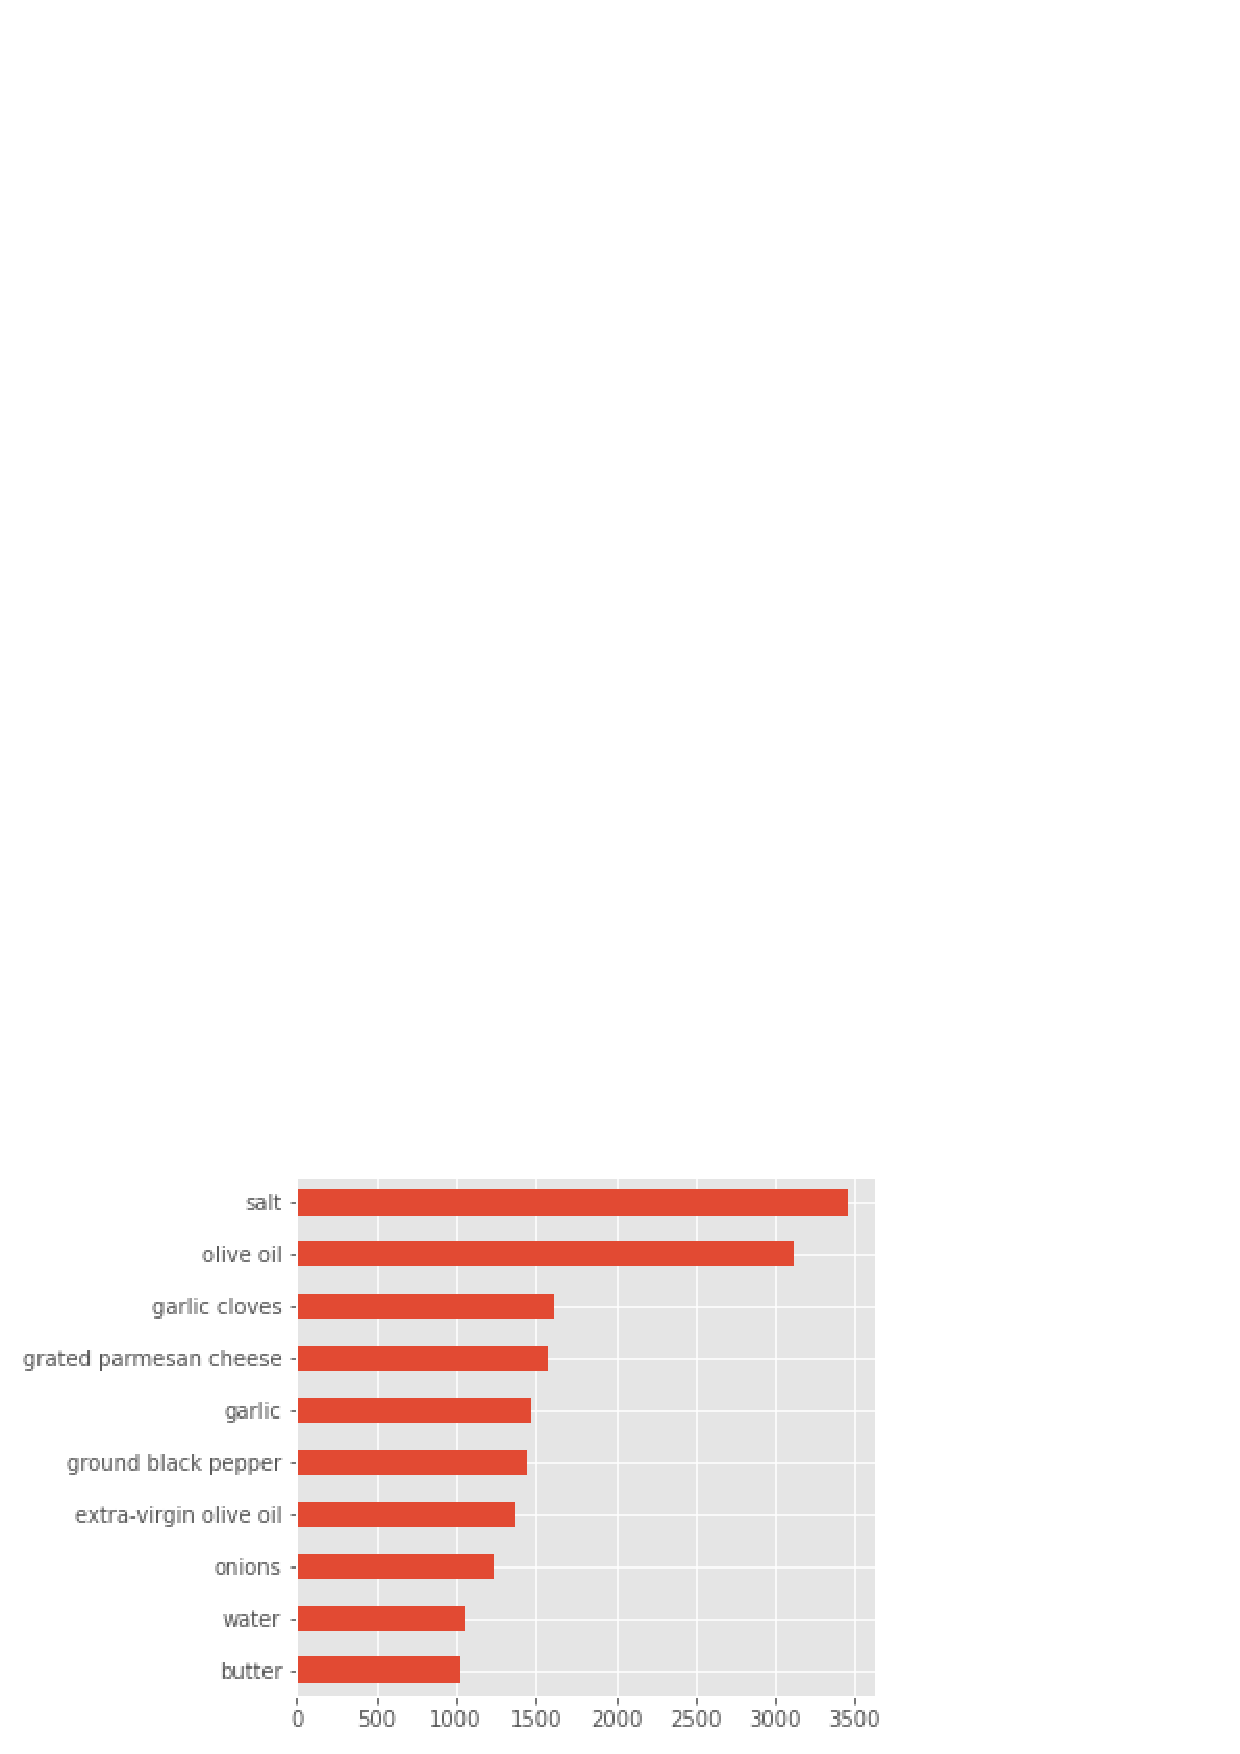
\includegraphics[width=0.5\textwidth]{pic1/italian.png} 
    \end{minipage}
   
}
\block{Data cleaning}{
   
    \begin{itemize}                            
        \item
        Since dishes contain a large number of ingredients, and since the same ingredients can vary in numbers, tenses, and so on, we considered sifting through a potatos to remove any such differences
    \end{itemize}
   
    
}
% SECOND column
\column{0.5}
 %Second column with first block's top edge aligned with with previous column's top.

%%%%%%%%%% -------------------------------------------------------------------- %%%%%%%%%%
%%%%%%%%%% -------------------------------------------------------------------- %%%%%%%%%%
% Second column - first block

%%%%%%%%%% -------------------------------------------------------------------- %%%%%%%%%%
\block{Feature extraction}{
   
    \begin{itemize}  
                                  
        \item We convert the ingredients of the dish into a numerical feature vector.Consider that most dishes include salt, water, sugar, butter, etc,We will consider weighting the seasonings according to the occurrence times of the seasonings, that is, the more the occurrence times of the condiments, the lower the discriminability of the condiments.The feature we adopt is TF-IDF.
        \item We can get the top 5 characteristics:\lbrack'greek','southern\_us','filipino','indian','indian'\rbrack
        \item The first five data in train\_tfidf:
        \lbrack\lbrack0. 0. 0. ... 0. 0. 0.\rbrack\\
        \lbrack0. 0. 0. ... 0. 0. 0.\rbrack\\
        \lbrack0. 0. 0. ... 0. 0. 0.\rbrack\\
        \lbrack0. 0. 0. ... 0. 0. 0.\rbrack\\
        \lbrack0. 0. 0. ... 0. 0. 0.\rbrack\rbrack
    \end{itemize}
    
}

%%%%%%%%%% -------------------------------------------------------------------- %%%%%%%%%%
\block{Validation set partitioning}{
   
    \begin{itemize}  
                                    
       \item 
        The training set is divided into a new training set and a validation set by calling train\_test\_split function, which is convenient for the subsequent accuracy observation of the model.
       \item
        
        1.Use train\_tfidf and train\_targets as input variables for train\_test\_split\\
        2.The test\_size is set to 0.2, 20$\%$ of the validation set is divided, and 80$\%$ of the data is reserved for the new training set.\\
        3.Set the random\_state random seed to ensure that the same partition results are obtained every time you run it.
     
    \end{itemize}
    
}
%%%%%%%%%% -------------------------------------------------------------------- %%%%%%%%%%
\block{raining Model}{
   
    \begin{itemize}  
                                    
        \item 
        Invoke the logistic regression model in sklearn.
       
       \item 
         1.GridSearchCV is imported from sklearn.model\_selection, and the parameters are automatically searched. As long as the parameters are typed in, the best results and parameters can be given. \\
         2.Define the parameters variable: Create a dictionary for the C parameters, whose values are an array from 1 to 10;\\
         3.Define the classifier variable: Create a classification function using the imported LogisticRegression;\\
         4.Define Grid variables: Create a grid search object using the imported GridSearchCV;Pass the variables 'classifier', 'parameters' as arguments to the object constructor;
         \item 
         After the model training, we calculated the prediction results of the model on the validation set X\_VALID, and calculated the prediction accuracy of the model .
         \item 
         The score on the validation set is: 0.7958516656191075.
    \end{itemize}
    
}

% Second column - second block
%%%%%%%%%% -------------------------------------------------------------------- %%%%%%%%%%
\block[titlewidthscale=1, bodywidthscale=1]
{Predictive test set}
{
\begin{itemize} 
  \item
  Test set test\_tfidf is predicted by the model grid, and then the predicted results are viewed.\\
  The predicted number of test sets is 9944  
\end{itemize}
\begin{minipage}{1\linewidth}
    \flushleft
    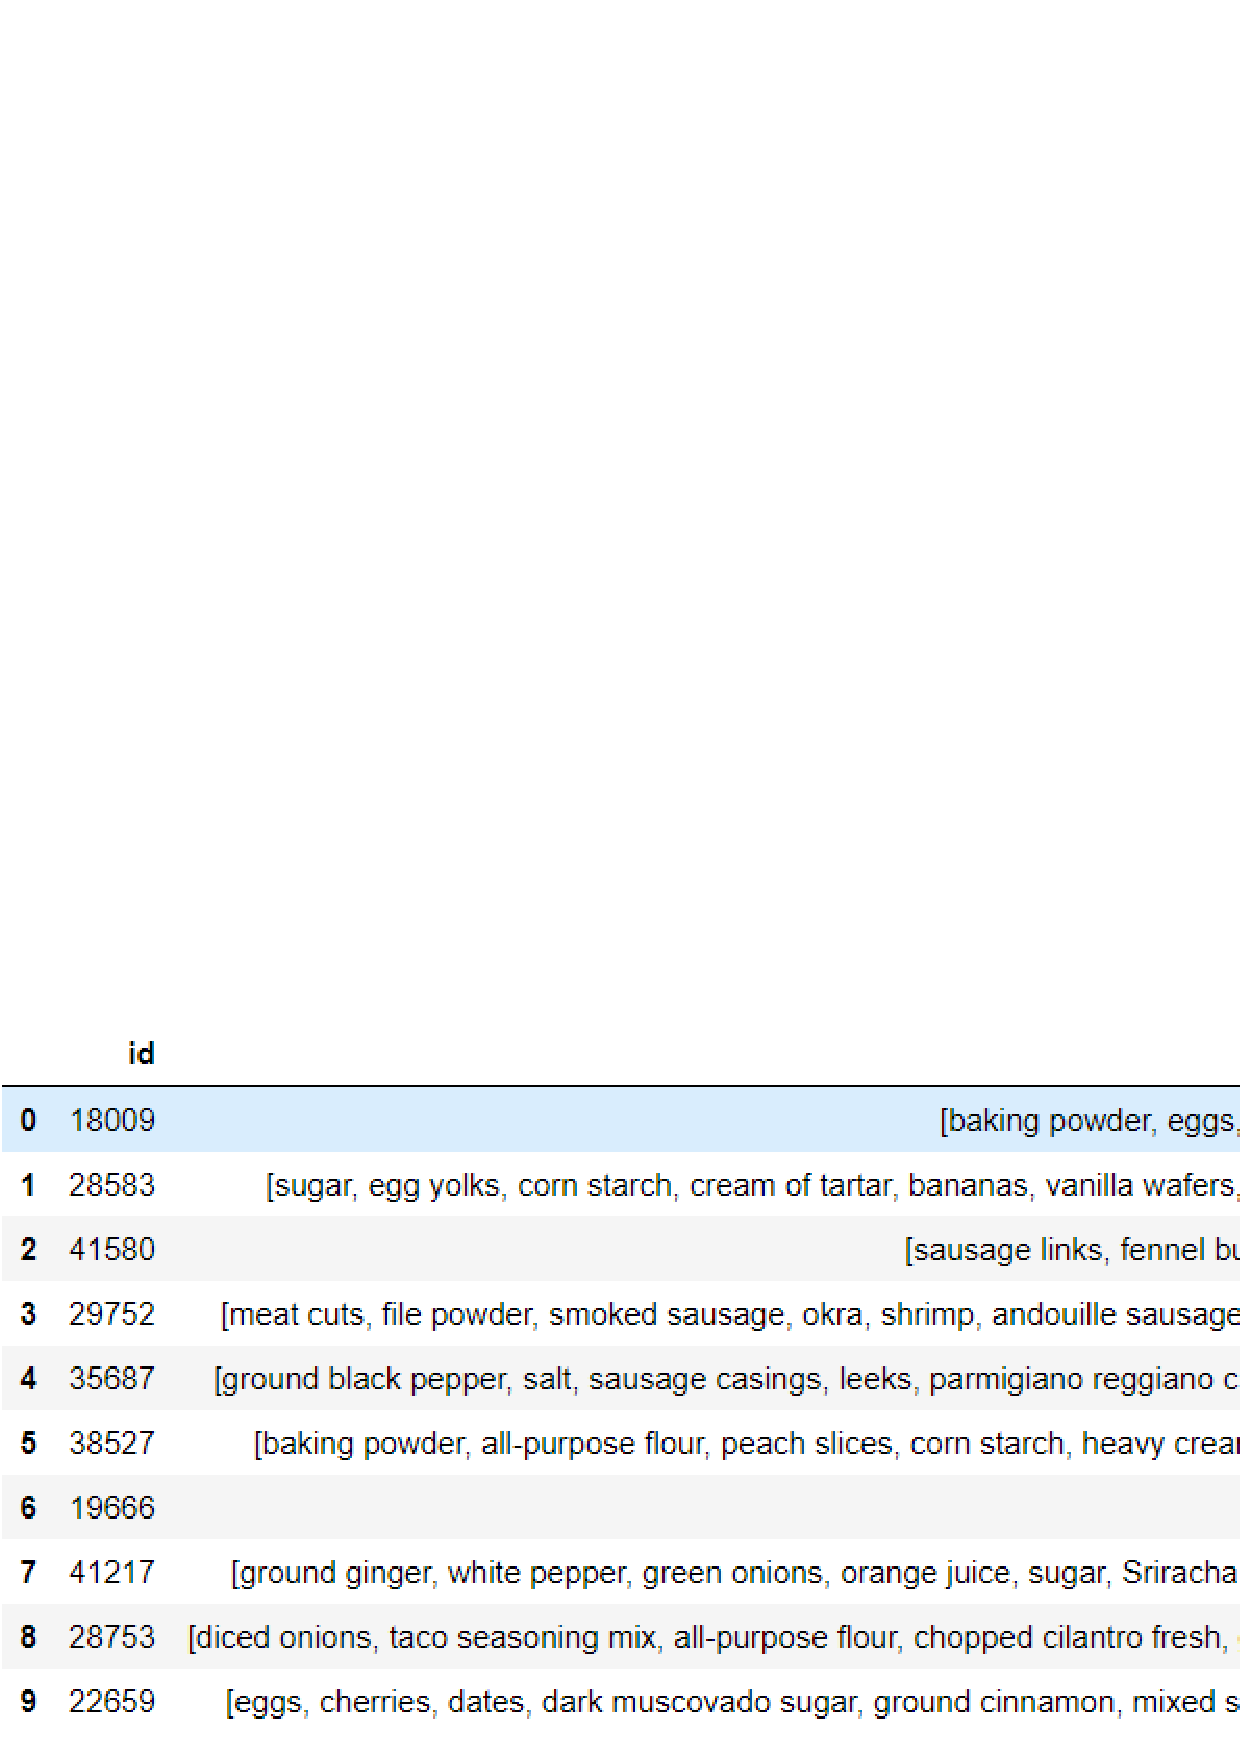
\includegraphics[width=0.5\textwidth]{pic1/result.png} 
\end{minipage}
}
%%%%%%%%%% -------------------------------------------------------------------- %%%%%%%%%%


% Bottomblock
%%%%%%%%%% -------------------------------------------------------------------- %%%%%%%%%%
\colorlet{notebgcolor}{blue!20}
\colorlet{notefrcolor}{blue!20}
\note[targetoffsetx=8cm, targetoffsety=-5cm, angle=30, rotate=15,
radius=2cm, width=.26\textwidth]{
Acknowledgement
\begin{itemize}
    \item
    International Cooperation Project (Y7Z0511101)
    of IIE,
    Chinese Academy of Sciences
 \end{itemize}
}

%\note[targetoffsetx=8cm, targetoffsety=-10cm,rotate=0,angle=180,radius=8cm,width=.46\textwidth,innersep=.1cm]{
%Acknowledgement
%}

%\block[titlewidthscale=0.9, bodywidthscale=0.9]
%{Acknowledgement}{
%}
%%%%%%%%%% -------------------------------------------------------------------- %%%%%%%%%%

\end{columns}


%%%%%%%%%% -------------------------------------------------------------------- %%%%%%%%%%
%[titleleft, titleoffsetx=2em, titleoffsety=1em, bodyoffsetx=2em,%
%roundedcorners=10, linewidth=0mm, titlewidthscale=0.7,%
%bodywidthscale=0.9, titlecenter]

%\colorlet{noteframecolor}{blue!20}
\colorlet{notebgcolor}{blue!20}
\colorlet{notefrcolor}{blue!20}
\note[targetoffsetx=-13cm, targetoffsety=-13cm,rotate=0,angle=180,radius=8cm,width=.96\textwidth,innersep=.4cm]
{
\begin{minipage}{0.3\linewidth}
\centering
\includegraphics[width=24cm]{logos/tulip-wordmark.eps}
\end{minipage}
\begin{minipage}{0.7\linewidth}
{ \centering
 The $11^{th}$ International Conference on Knowledge Science,
  Engineering and Management (KSEM 2018),
  17-16/20/2020,Xi'an, China
}
\end{minipage}
}
%%%%%%%%%% -------------------------------------------------------------------- %%%%%%%%%%


\end{document}

%\endinput
%%
%% End of file `tikzposter-template.tex'.
